\chapter{Results}

\section{Torque estimation}
All four NN models were tested against various datasets. Using the angle data and 
physiological parameters of the user, actual torque was calculated. Then, model 
predicted torque was plotted against it.  

\subsection{Single dataset models}
As illustrated in Figures \ref{fig:ovc0g}, \ref{fig:ovc0gstops} and \ref{fig:ovc10kg} 
the $closed\_model$ beats the $open\_model$ in terms of accuracy but neither 
achieve satisfactory results for higher loads. In fact, these models were trained 
on a dataset where a load of 900g was used and they work best on datasets with 
similar loads. The biggest advantage of the $closed\_model$ over the $open\_model$ 
is its better performance on the dataset containing stops illustrated in Figure 
\ref{fig:ovc0gstops}.  
\begin{figure}[htbp]
  \centering
  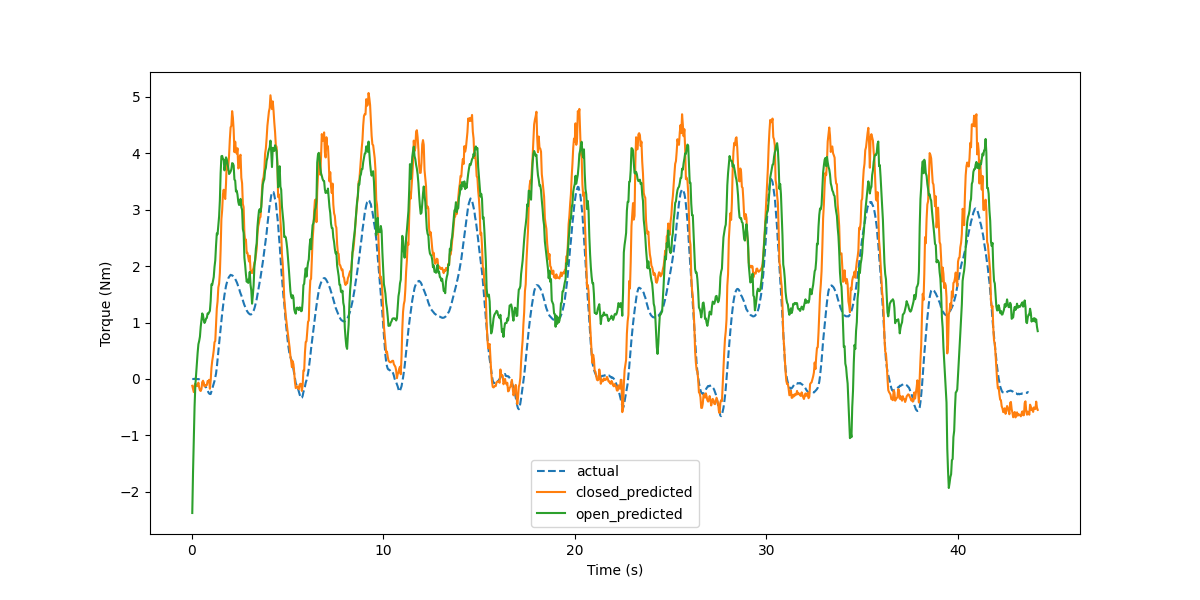
\includegraphics[width=\textwidth]{open_vs_closed_0g.png}
  \caption{No load}
  \label{fig:ovc0g}
\end{figure}
\begin{figure}[htbp]
  \centering
  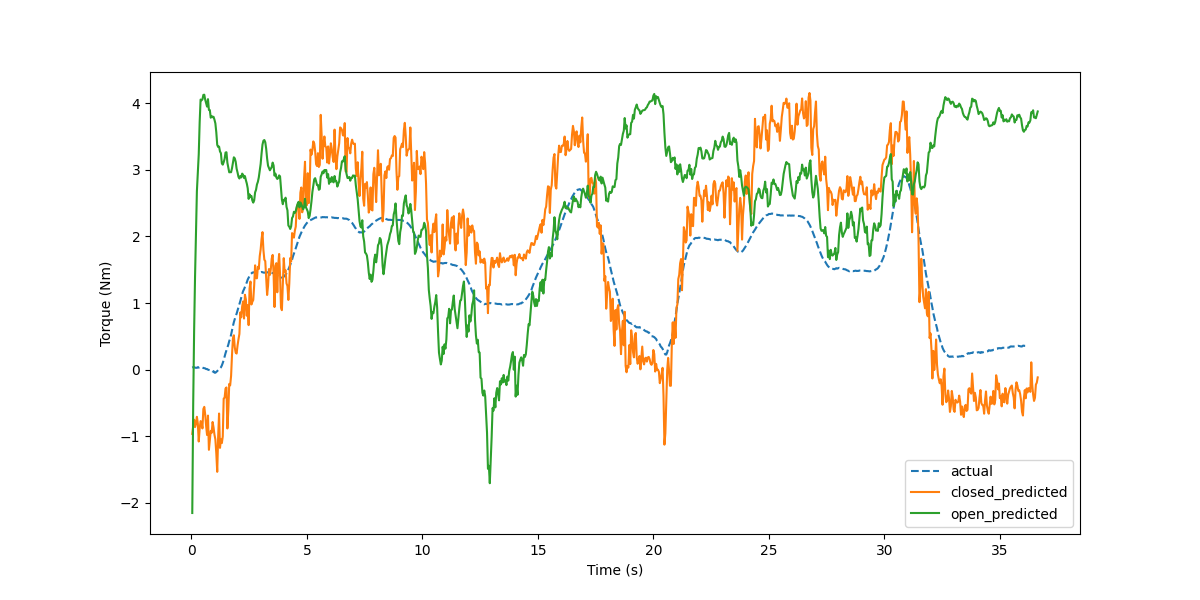
\includegraphics[width=\textwidth]{open_vs_closed_0g_stops.png}
  \caption{No load with stops}
  \label{fig:ovc0gstops}
\end{figure}
\begin{figure}[htbp]
  \centering
  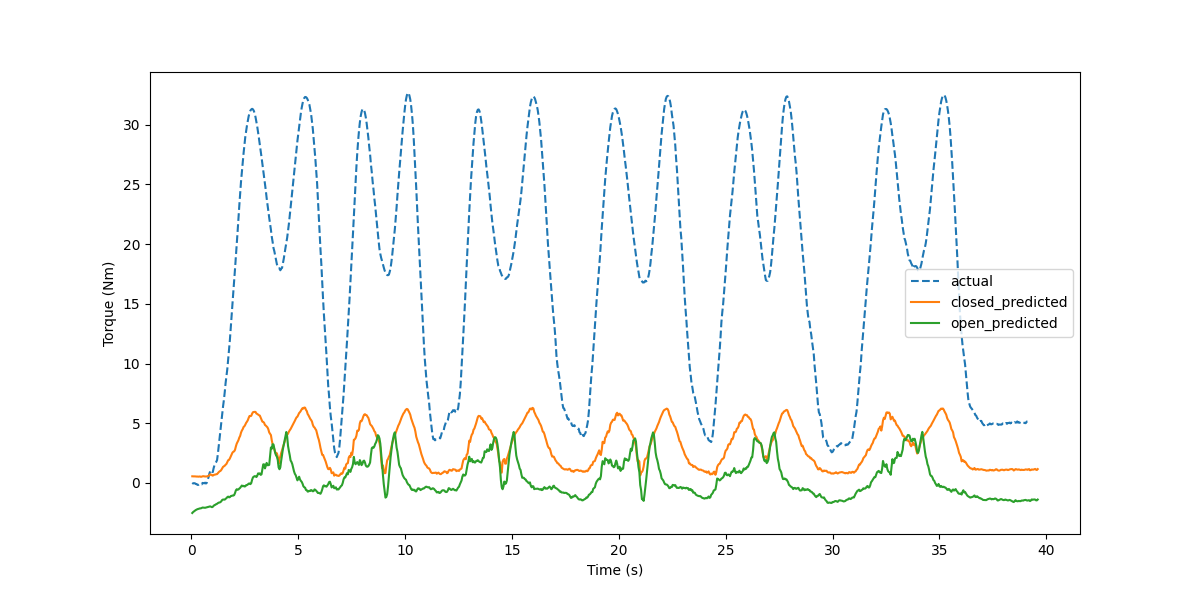
\includegraphics[width=\textwidth]{open_vs_closed_10kg.png}
  \caption{10kg load}
  \label{fig:ovc10kg}
\end{figure}
\FloatBarrier

\subsection{Multi-dataset models}
Models trained on all initial datasets showed no advantage over the first two 
models. As illustrated in Figures \ref{fig:movc0g}, \ref{fig:movcstops} and \ref{fig:movc10kg}, 
$multi\_open\_model$ and $multi\_closed\_model$ performed worse than their 
single-dataset counterparts.  

\begin{figure}[htbp]
  \centering
  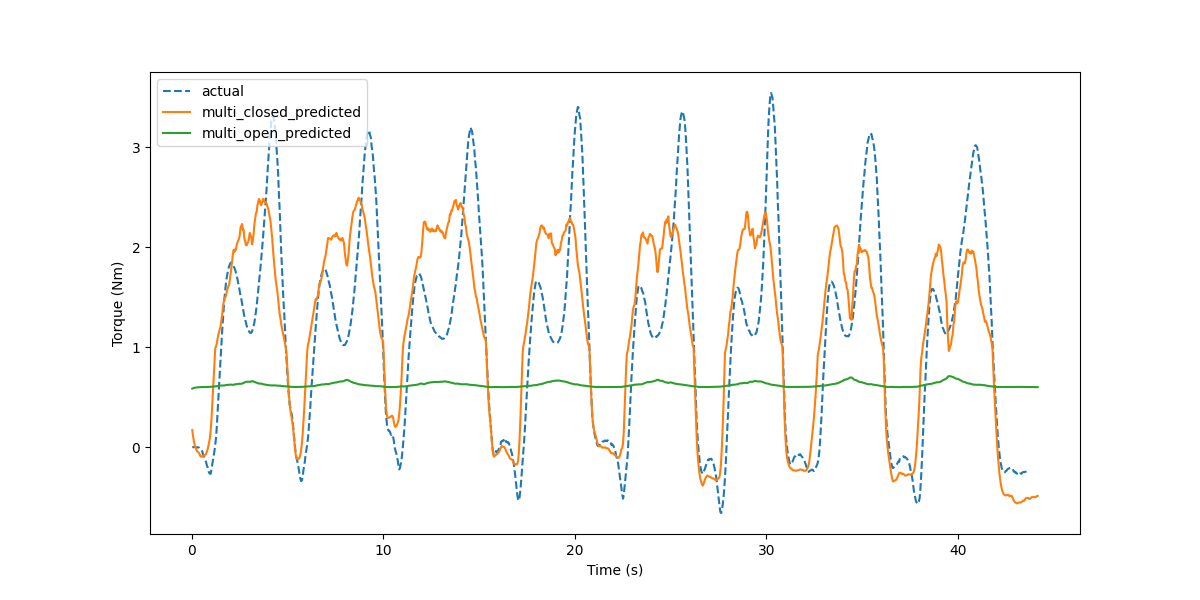
\includegraphics[width=\textwidth]{multi_open_vs_closed_0g.png}
  \caption{No load}
  \label{fig:movc0g}
\end{figure}
\begin{figure}[htbp]
  \centering
  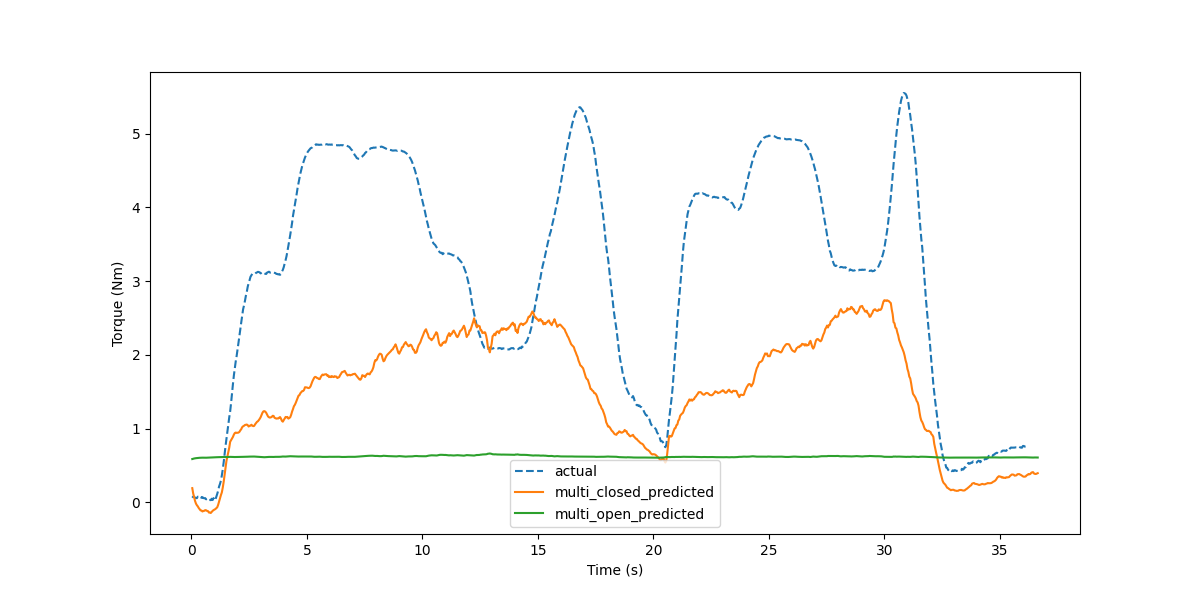
\includegraphics[width=\textwidth]{multi_open_vs_closed_stops.png}
  \caption{No load with stops}
  \label{fig:movcstops}
\end{figure}
\begin{figure}[htbp]
  \centering
  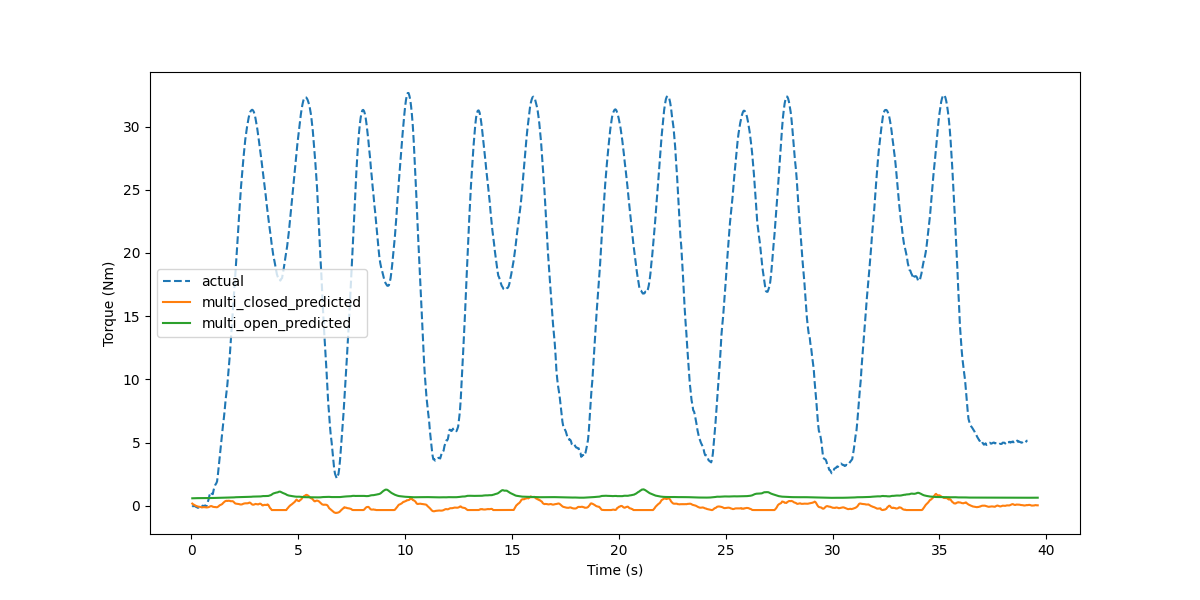
\includegraphics[width=\textwidth]{multi_open_vs_closed_10kg.png}
  \caption{10kg load}
  \label{fig:movc10kg}
\end{figure}
\FloatBarrier

\section{Orthosis control}
\subsection{Experimental setup}
The experimental setup is illustrated in Figure \ref{fig:setup}. The motor driver 
is first connected to the PC via USB, then the motor is securely tightened to the 
table surface and connected to the driver. The power supply is then also connected 
to the driver via a twisted pair power cable. Finally, the rope is tightened to 
prepare the system for testing.  

\begin{figure}[htbp]
  \centering
  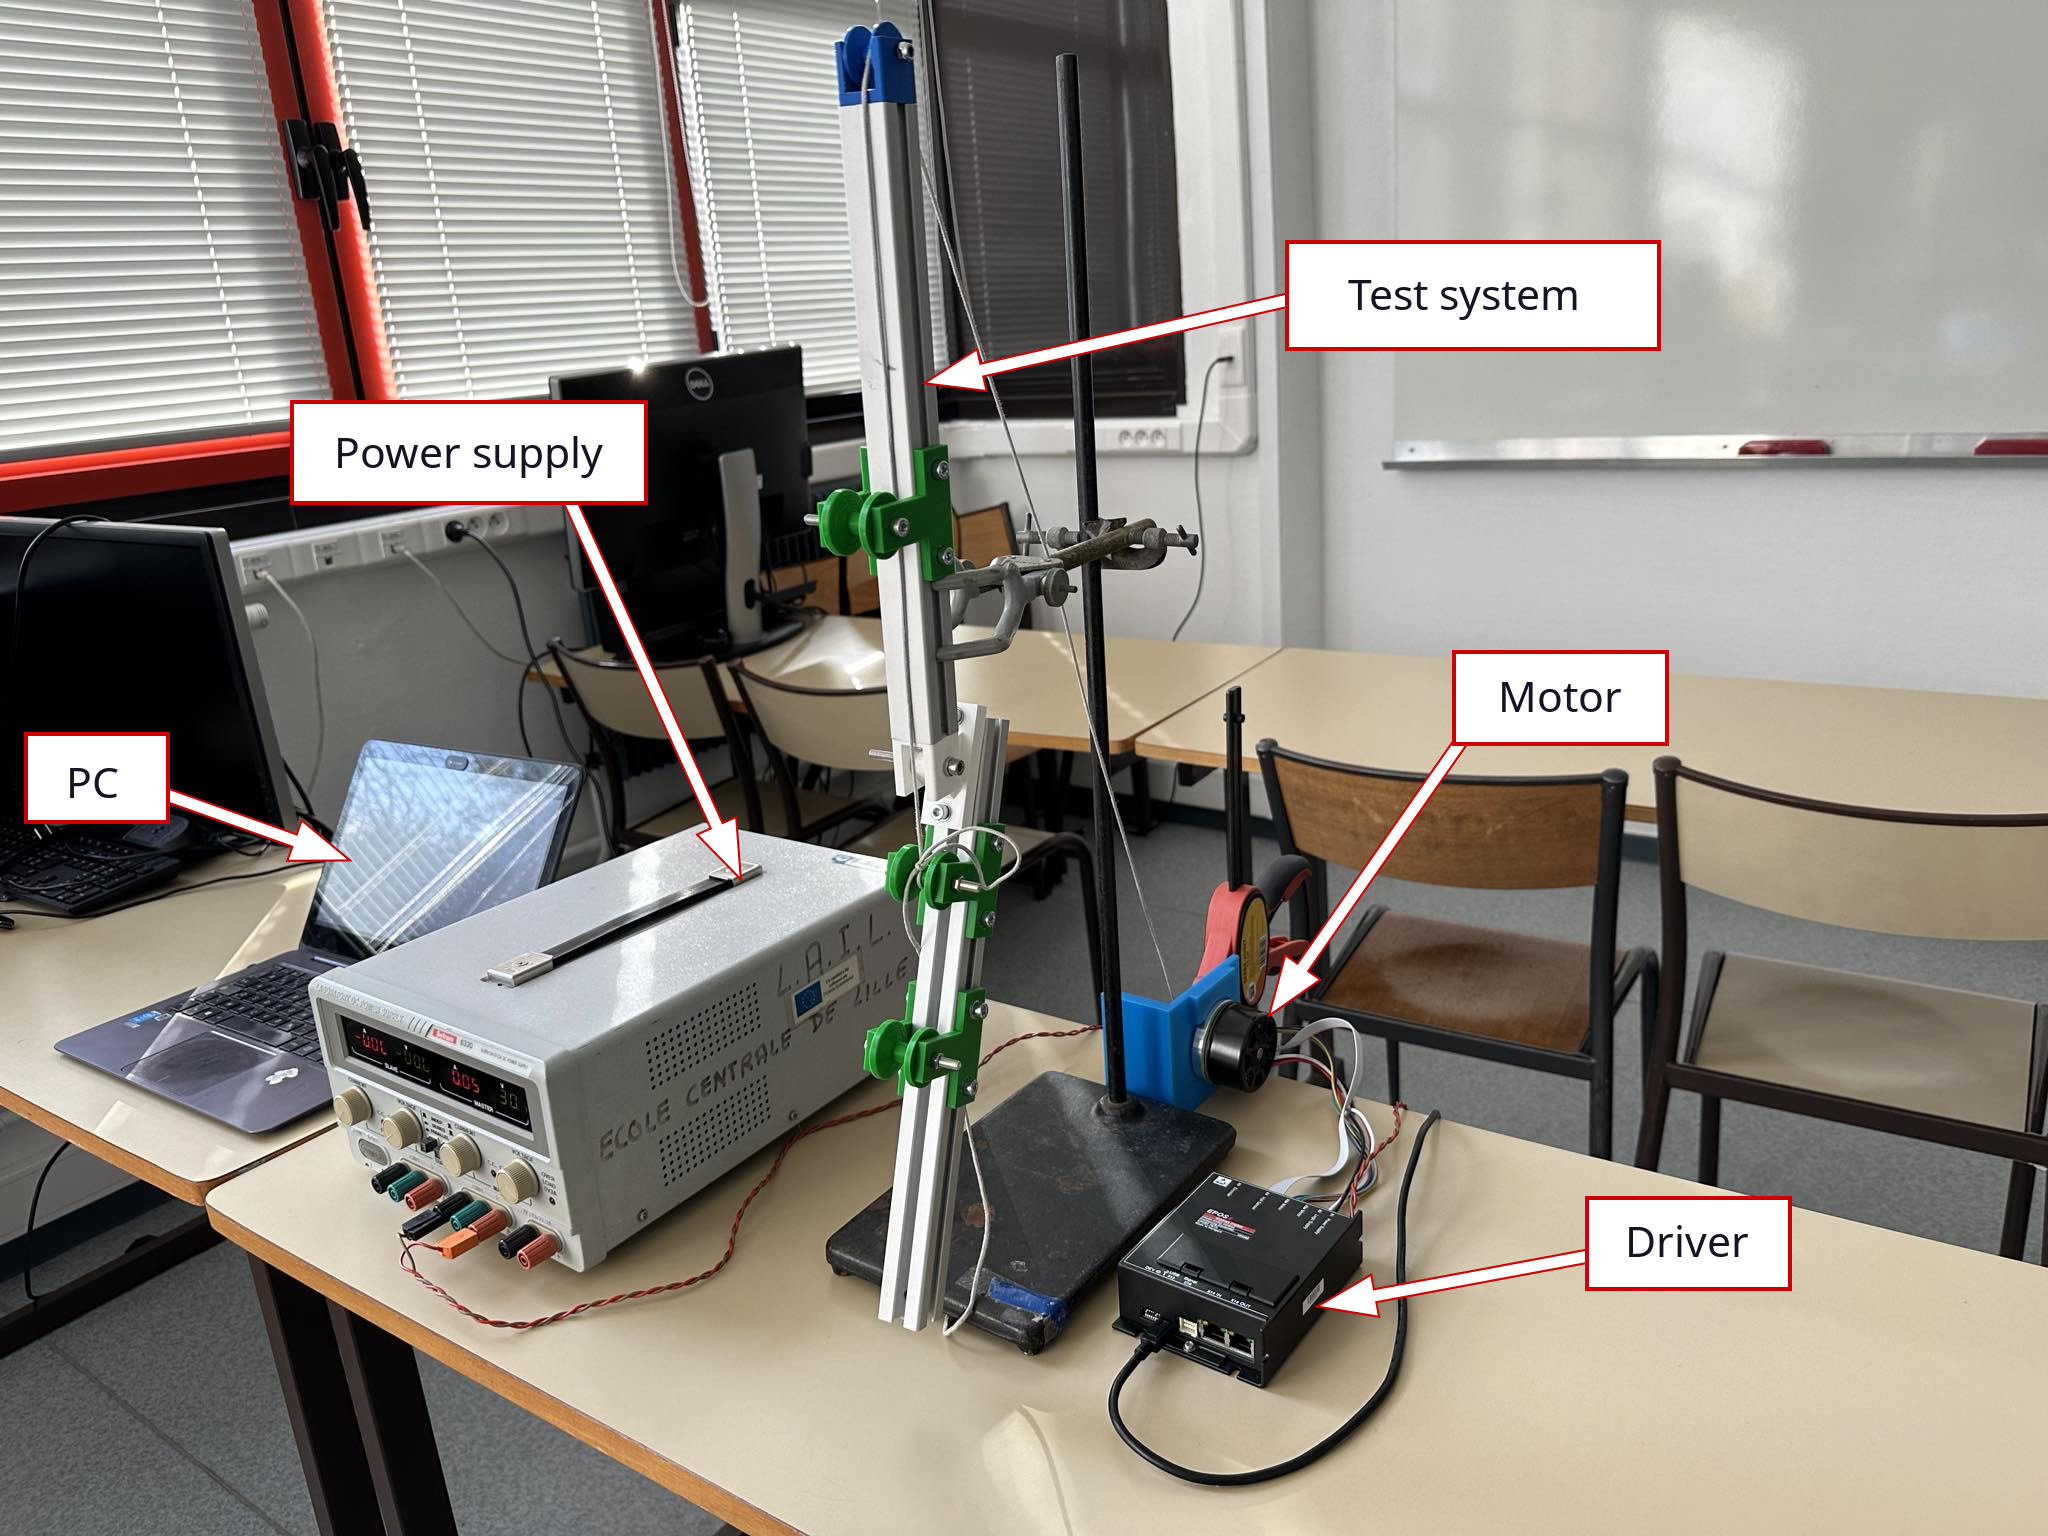
\includegraphics[width=0.6\textwidth]{setup.png}
  \caption{Experimental setup}
  \label{fig:setup}
\end{figure}

As shown in Figure \ref{fig:sensor_system_sock}, the sensor system was installed on a sock by sewing 
each component individually. Thus, a soft orthosis system could be simulated 
for control purposes. 

\begin{figure}[htbp]
    \centering
    \begin{subfigure}{0.3\textwidth}
        \centering
        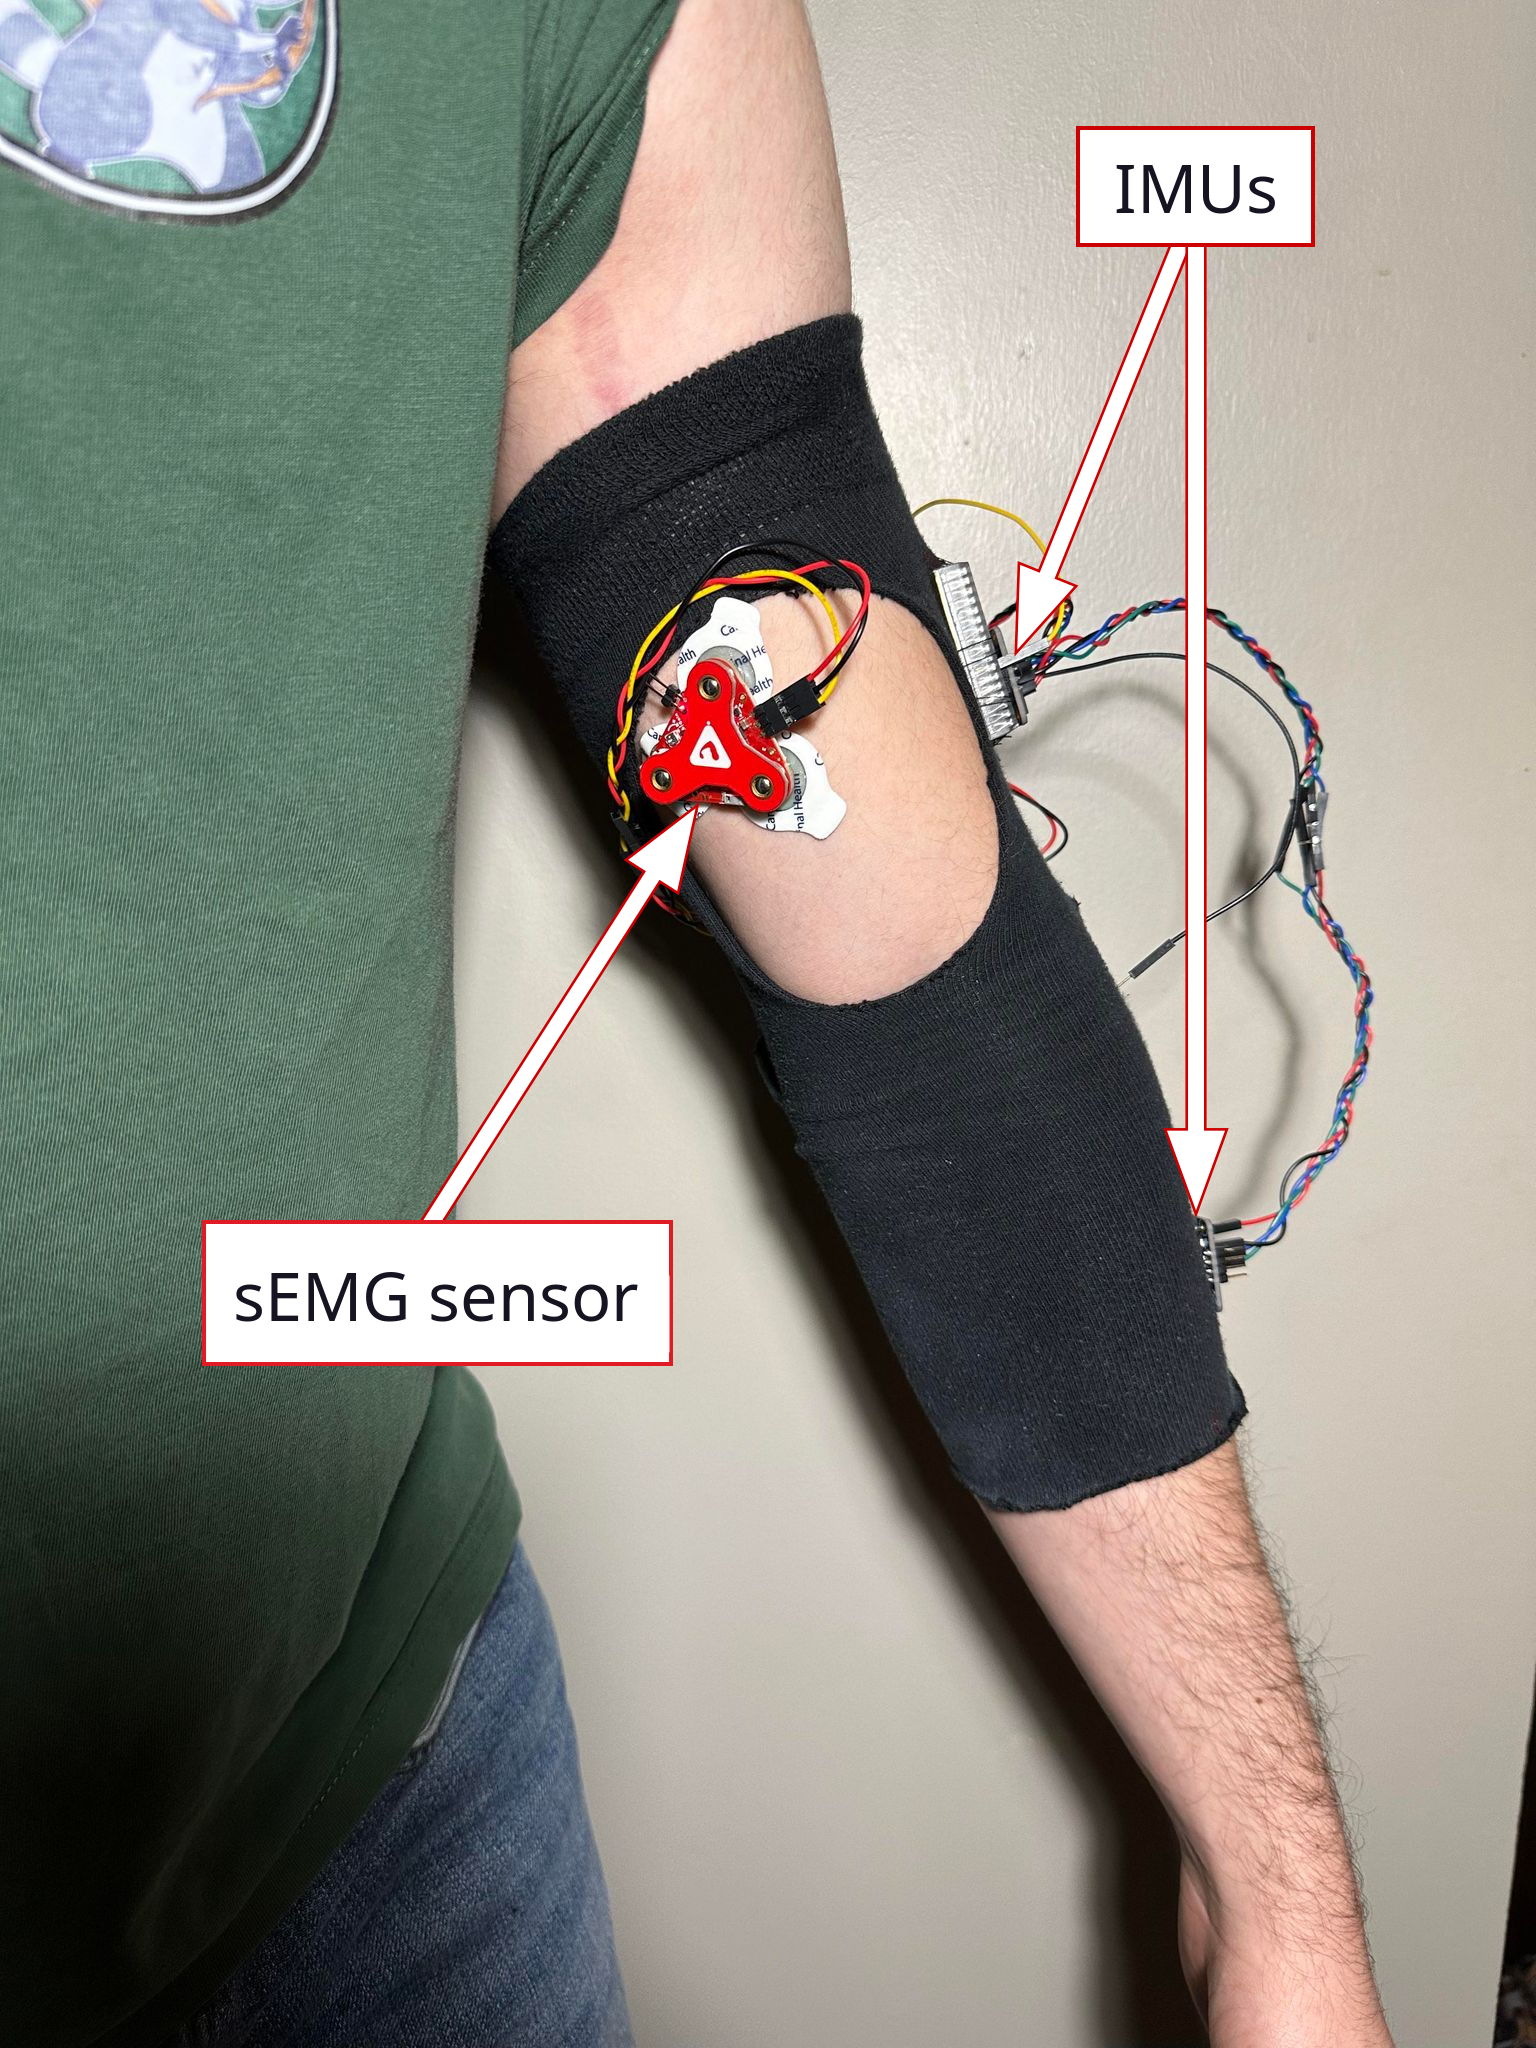
\includegraphics[width=\linewidth]{front_view.png}
        \caption{Front}
    \end{subfigure}
    \begin{subfigure}{0.3\textwidth}
        \centering
        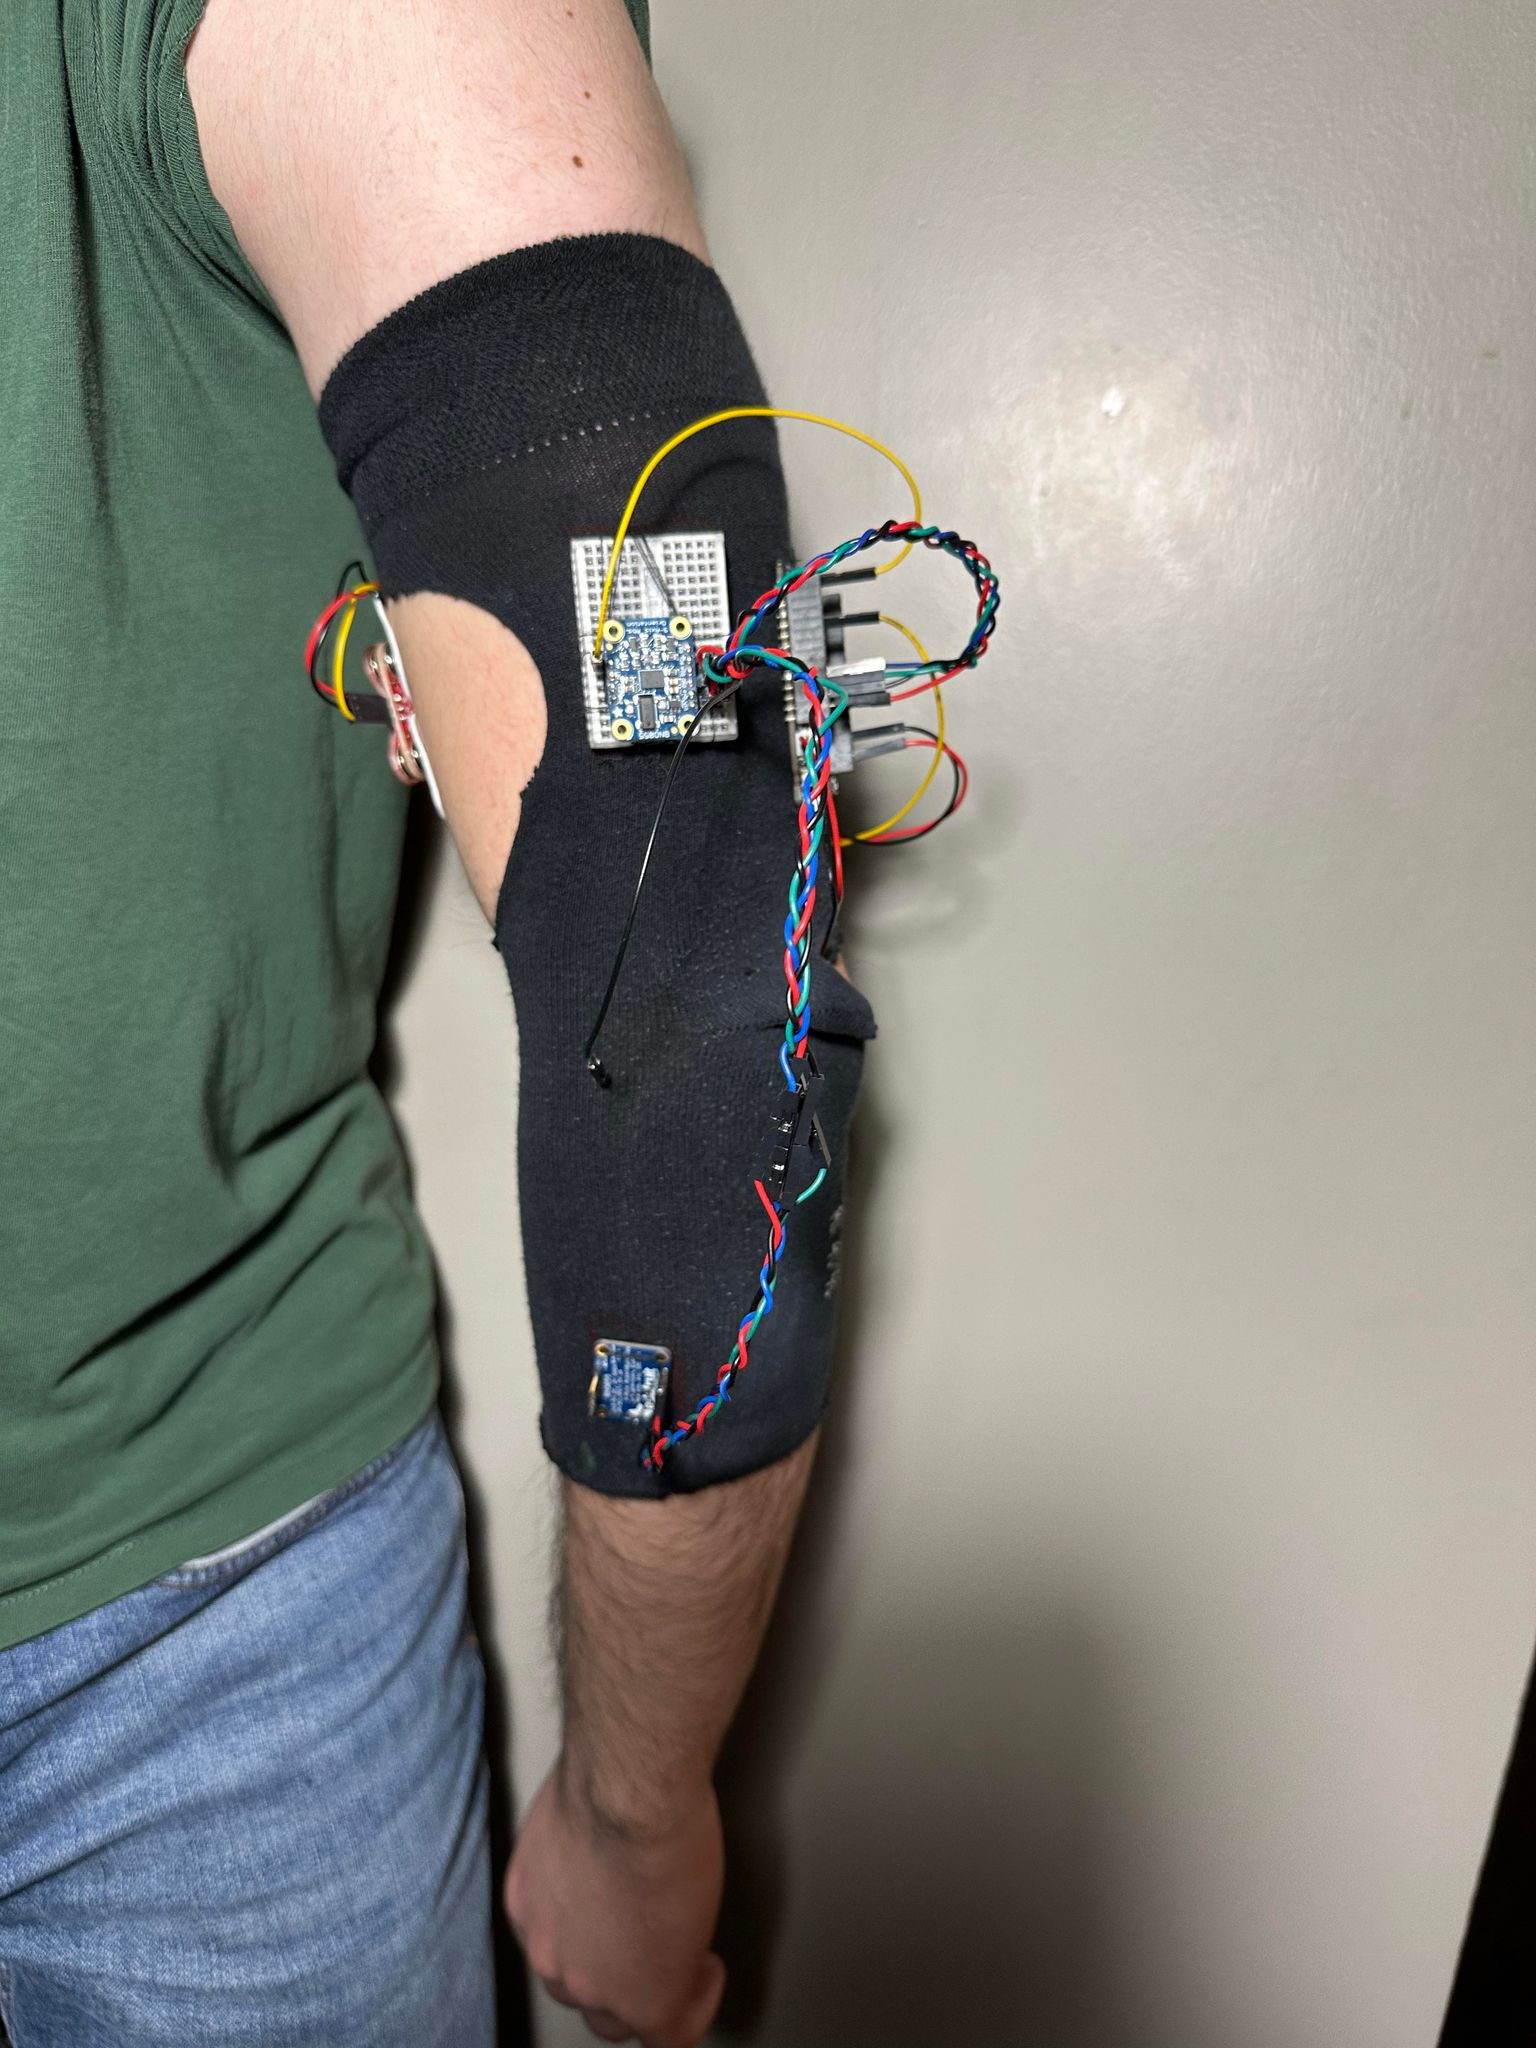
\includegraphics[width=\linewidth]{side_view.jpg}
        \caption{Side}
    \end{subfigure}
    \begin{subfigure}{0.3\textwidth}
        \centering
        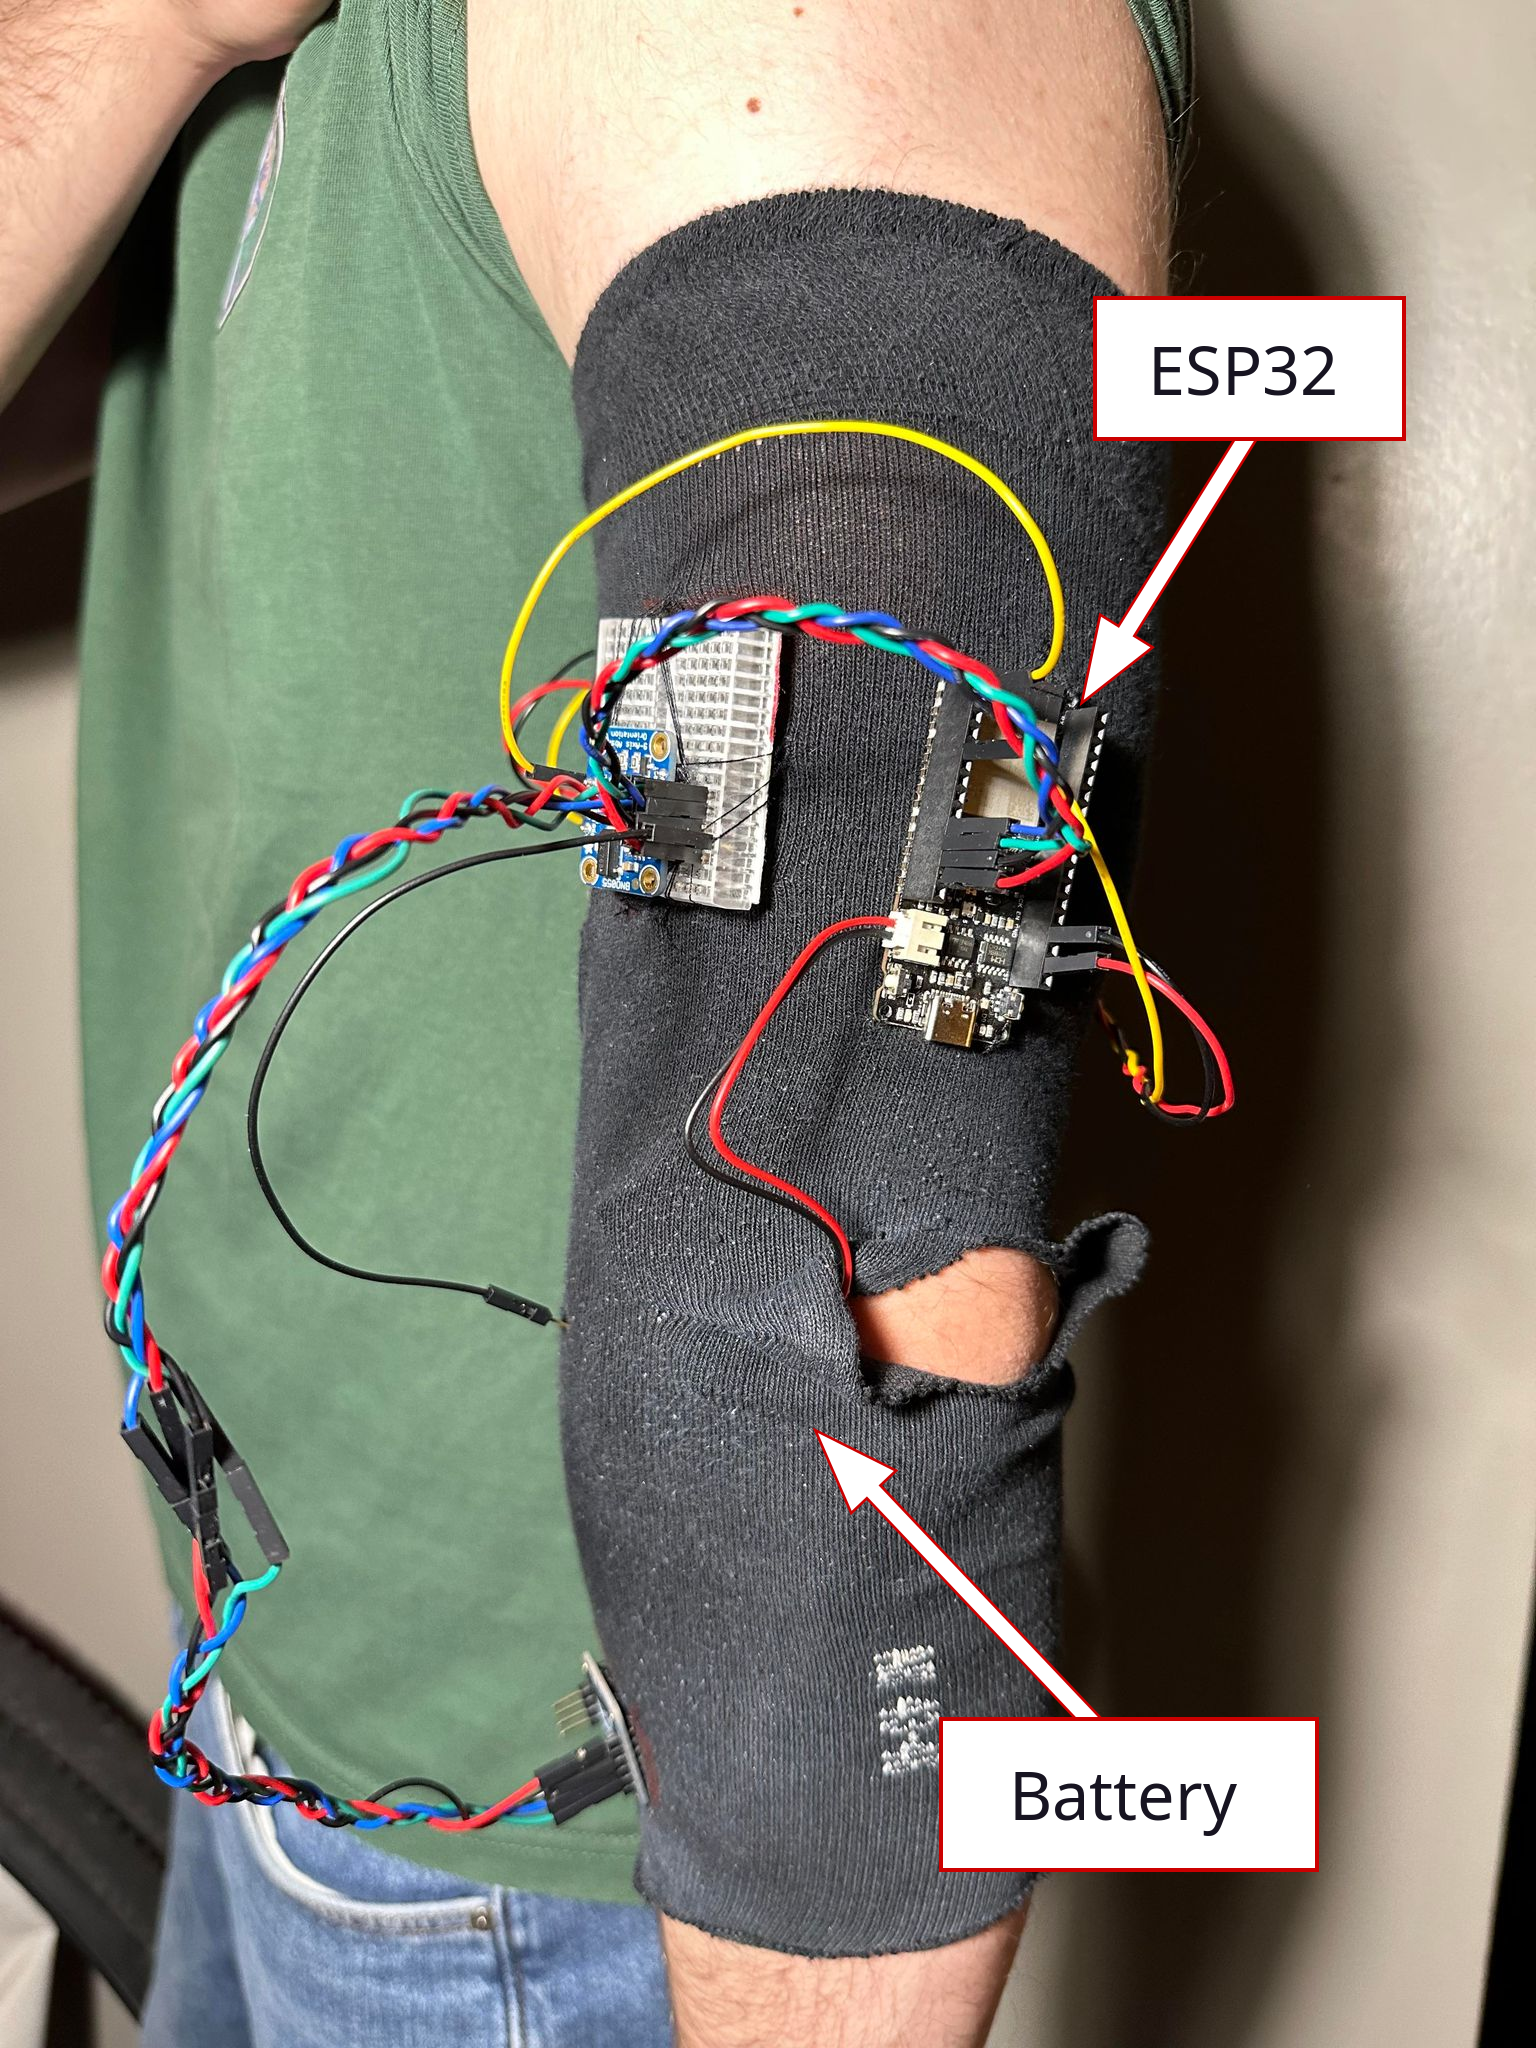
\includegraphics[width=\linewidth]{back_view.png}
        \caption{Back}
    \end{subfigure}
    \caption{
      Control system on a sock
    }
    \label{fig:sensor_system_sock}
\end{figure}

\FloatBarrier
\subsection{Experimental results}
The control strategy shown in Figure \ref{fig:control_diagram} 
did not produce the desired results based on visual evaluation.  

The goal was that the test system shown in Figure \ref{fig:setup} 
starts applying an assistive torque as soon as motion intention is detected and 
stops providing this assistance as soon as that intention disappears. However, 
utilizing the devised control strategy only resulted in sporadic flexion of the 
test system as the identified torque values peaked too fast and too high, on top 
of arriving well after the user had already begun the motion.  

A test where the test system was controlled by an even simpler control strategy 
shown in Figure \ref{fig:simplified_control_diagram} was successfully conducted. This test consisted in 
controlling the test system proportionally to the user's sEMG signal. Current 
command values were saturated for safety. The result was flexion of the test 
system that could be controlled by the contraction of the user's biceps through 
proportional current control.

\begin{figure}[htbp]
    \centering
    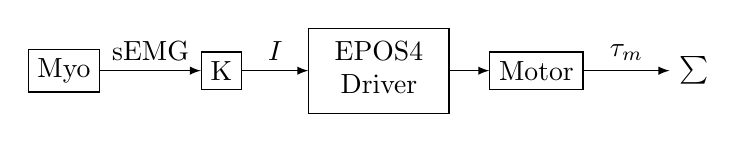
\begin{tikzpicture}[auto, node distance=2cm,>=latex]
        \tikzstyle{block} = [draw, rectangle]
        
        \node [block, draw] (input) at (0,0) {Myo};
        \node [block, right of=input, node distance=2cm] (gain) {K};
        \node [block, right of=gain, node distance=2cm] (driver) {
          \begin{tabular}{c}
            EPOS4\\ 
            Driver
          \end{tabular}
        };
        \node [block, right of=driver, node distance=2cm] (motor) {Motor};
        \node [right of=motor] (sys) {$\sum$};

        \draw [->] (input) -- node[above] {sEMG} (gain);
        \draw [->] (gain) -- node[above] {$I$} (driver);
        \draw [->] (driver) -- (motor);
        \draw [->] (motor) -- node[above] {$\tau_m$} (sys);
    \end{tikzpicture}
    \caption{
      Simplified Control Diagram - $K$ is an arbitrary gain 
    }
    \label{fig:simplified_control_diagram}
\end{figure}
\FloatBarrier
